\documentclass[10pt,letterpaper]{article}

\usepackage[utf8]{inputenc}
\usepackage[T1]{fontenc}
\usepackage{graphicx}
\usepackage{xcolor}
\usepackage{geometry}
\usepackage{titlesec}
\geometry{margin=1in}
\setlength{\parindent}{1.5em}
\setlength{\parskip}{0pt}
\setlength{\textfloatsep}{4pt}
\setlength{\floatsep}{4pt}
\setlength{\intextsep}{4pt}
\titleformat{\section}{\large\bfseries}{}{0pt}{}
\titlespacing*{\section}{0pt}{0.55ex}{0.3ex}

\begin{document}
\begin{center}
{\Large\bfseries Structure Before Scale: Accuracy, Uncertainty, and Procedural Stability Across Seven NFL Tracking Problems\par}
\vspace{0.25em}
Jonathan Pipping-Gam\'on\\
\textit{Department of Statistics \& Data Science, University of Pennsylvania}\\
Ron Yurko\\
\textit{Department of Statistics \& Data Science, Carnegie Mellon University}
\end{center}

\section*{Introduction}

Football tracking releases contain many player-frames but comparatively few independent games. Players, frames, and plays from the same contest share personnel, tactics, weather, and game state, so a model comparison based on one split can overstate both the available information and the dependability of a reported winner. We therefore ask a different question from an ordinary leaderboard comparison: which representation is sample-efficient for the mathematical structure of a football problem, and how reliably does the complete modeling procedure perform when the available games change?

We organize seven NFL Big Data Bowl prediction problems along three distinct axes. \textbf{Predictive accuracy or distributional skill} measures performance on the native task. \textbf{Uncertainty quality and concentration} asks whether calibrated intervals, sets, or trajectory tubes are informative rather than merely wide. \textbf{Procedural stability} measures variation across complete game-level reruns, including new partitions, nested samples, validation splits, initialization, and optimization. These outcomes need not identify the same preferred model.

The completed BDB2020 rushing-yards study is the confirmatory discovery reported here. BDB2021--2026 form a prospectively specified, result-blind suite spanning ordered distributions, temporal relational classification, focal-player and matchup classification, and social trajectory forecasting. This evidence boundary is important: no later-year performance result is claimed in this abstract.

\section*{Confirmatory Study Design}

The BDB2020 cohort contains 31,007 rushing plays from 688 games. Each of 100 paired whole-study reruns uses a season-stratified game split for training, calibration, and testing, with six nested training anchors of 20, 40, 80, 160, 240, and 360 games. Four frozen procedures are compared at every anchor: L2 one-vs-rest logistic regression and LightGBM on deterministic tracking summaries, a distributional Zoo CNN on a defender-by-offender pair grid, and a Set Transformer on player tokens. The resulting main grid contains 2,400 fitted cells.

Every procedure predicts an 80-class rushing-yard probability distribution. Continuous Ranked Probability Score (CRPS; lower is better) is primary. A locked locally weighted conformal procedure expands central model intervals using held-out calibration plays; empirical 90\% coverage and interval width are interpreted jointly, because a narrow interval is not useful if it undercovers. Sharpness claims require both models to clear the simultaneous coverage gate. All splitting is game-level, and the empirical 10th--90th percentile across 100 complete reruns describes whole-procedure variation rather than uncertainty for an individual play. Paired repeat-block inference preserves the common splits when comparing models.

The checksum-validated final receipt contains 3,000 unique fitted cells: 2,400 from the confirmatory main grid and 600 from a completed, pre-specified tuning sensitivity. Its stage-one decision triggered the planned extension to 50 paired reruns at 20, 160, and 360 games. The sensitivity is a separate evidence layer rather than part of the main grid.

\newpage
\section*{Confirmatory Findings}

\begin{figure}[t]
\centering
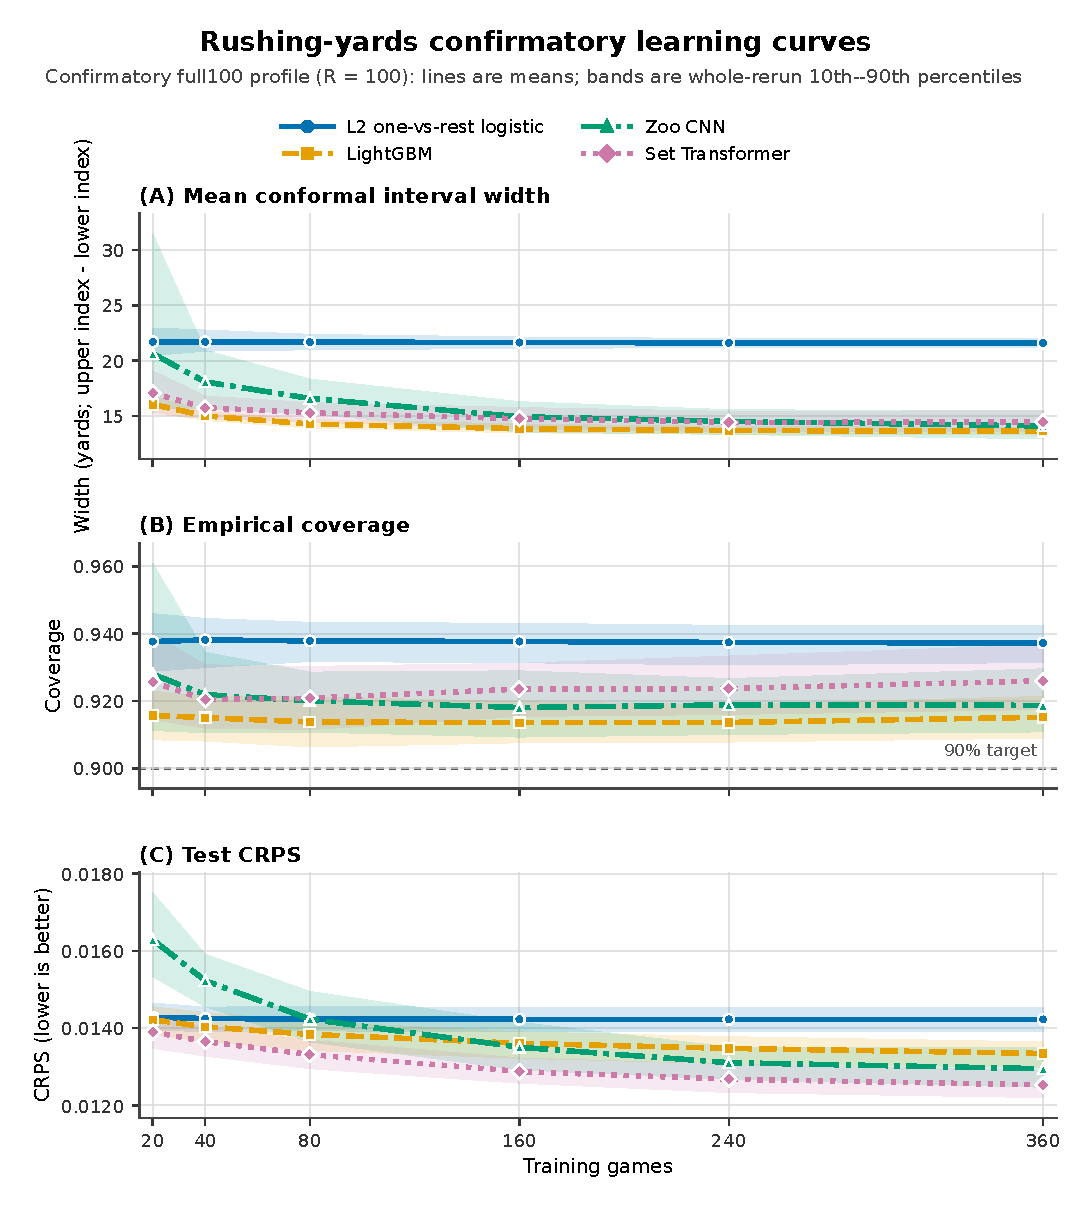
\includegraphics[width=0.42\linewidth]{../results/rushing/full100-confirmatory-20260820/final/main/rushing_confirmatory_100_learning_curves.pdf}
\caption{Confirmatory BDB2020 ($R=100$): means and whole-rerun 10th--90th percentile bands. Width and coverage use the locked 90\% interval; lower CRPS is better.}
\label{fig:full100}
\end{figure}

The Set Transformer has the lowest mean CRPS and meets the pre-specified simultaneous ``supported best'' rule against all three comparators at every training anchor. The result is already present at 20 games: mean CRPS is 0.013899 for the Transformer, 0.014218 for LightGBM, 0.014285 for logistic regression, and 0.016290 for the Zoo CNN. At 360 games the corresponding means are 0.012528, 0.013344, 0.014225, and 0.012947.

Accuracy does not settle the model choice. At 360 games, all four procedures clear the controlled-coverage gate, and LightGBM is supported as sharper than the Transformer: their mean interval widths are 13.644 and 14.465 yards, respectively. Logistic regression attains higher observed coverage using intervals roughly seven yards wider than the Transformer's. Nor does nominal complexity order stability. At 20 games the Zoo CNN's width SD is 8.106 yards, versus 1.509 for the Transformer; at 360 games the Transformer's CRPS SD is 0.000258, below the CNN's 0.000437 and close to the tabular procedures.

The completed 50-rerun sensitivity supports precise headline tuning robustness. After retuning within the frozen grids, the Set Transformer remains the supported CRPS winner, while LightGBM remains the narrowest coverage-qualified procedure and is supported as sharper than the Transformer, at 20, 160, and 360 games. The final trigger remains true because a lower-order mean ranking and some pairwise uncertainty conclusions changed; robustness is not universal.

These findings replace the simple story that small samples favor simple models and neural models become worthwhile only with scale. The organizing principle is \emph{structure before scale}: sample efficiency depends on whether parameter sharing, invariance, and relational aggregation match the problem. Because the BDB2020 neural inputs differ, this study cannot isolate the effect of attention; the matched-token CNN remains a one-split post-hoc diagnostic.

\section*{Prospective Tests and Conclusion}

BDB2021--2026 prospectively test the structural explanation with five primary roles. Linear-Structure and Boosted-Structure share deterministic summaries. RelNet and AttnRelNet share inputs, frame history, graph, encoder, head, loss, tuning grid, and seeds, differing only in fixed versus attention-weighted aggregation. A Global Set Transformer shares the neural tokens, history, timing, context, head, loss, folds, and training protocol but replaces typed graph edges with global masked set attention. Each task adds a matched structure-removal comparison at 20 games and the largest anchor. Their planned 100-rerun results remain unobserved.

Completed evidence shows that the best distributional predictor need not give the sharpest calibrated interval and headline robustness can coexist with secondary changes: structure comes before scale.

\end{document}
